\documentclass{article}


\usepackage[utf8]{inputenc}
\usepackage{amssymb}
\usepackage{bm}
\usepackage[ruled,vlined]{algorithm2e}
\usepackage{hyperref}

\usepackage{graphicx}
\usepackage{float}
\usepackage{amsmath}
\usepackage{tikz}
\usepackage{lmodern}
\usepackage{subcaption}
\usepackage{bbm}
\usepackage{multirow}
\usetikzlibrary{positioning, backgrounds, fit, shapes.arrows}
\usetikzlibrary{decorations.markings}
\usetikzlibrary{shapes.geometric,shapes.symbols,fit,positioning,shadows}

\usepackage{amsthm}

\newtheorem{theorem}{Theorem}[section]
\newtheorem{corollary}{Corollary}[theorem]
\newtheorem{lemma}[theorem]{Lemma}
\newtheorem{prop}{Proposition}
\newtheorem{assumption}{Assumption}[section]

\makeatletter
\tikzstyle{dummy} = [coordinate]
\pgfkeys{/pgf/.cd,
  parallelepiped offset x/.initial=2mm,
  parallelepiped offset y/.initial=2mm
}
\pgfdeclareshape{parallelepiped}
{
  \inheritsavedanchors[from=rectangle] \inheritanchorborder[from=rectangle]
  \inheritanchor[from=rectangle]{north}
  \inheritanchor[from=rectangle]{north west}
  \inheritanchor[from=rectangle]{north east}
  \inheritanchor[from=rectangle]{center}
  \inheritanchor[from=rectangle]{west}
  \inheritanchor[from=rectangle]{east}
  \inheritanchor[from=rectangle]{mid}
  \inheritanchor[from=rectangle]{mid west}
  \inheritanchor[from=rectangle]{mid east}
  \inheritanchor[from=rectangle]{base}
  \inheritanchor[from=rectangle]{base west}
  \inheritanchor[from=rectangle]{base east}
  \inheritanchor[from=rectangle]{south}
  \inheritanchor[from=rectangle]{south west}
  \inheritanchor[from=rectangle]{south east}
  \backgroundpath{
\southwest \pgf@xa=\pgf@x \pgf@ya=\pgf@y
    \northeast \pgf@xb=\pgf@x \pgf@yb=\pgf@y
    \pgfmathsetlength\pgfutil@tempdima{\pgfkeysvalueof{/pgf/parallelepiped offset x}}
    \pgfmathsetlength\pgfutil@tempdimb{\pgfkeysvalueof{/pgf/parallelepiped offset y}}
    \def\ppd@offset{\pgfpoint{\pgfutil@tempdima}{\pgfutil@tempdimb}}
    \pgfpathmoveto{\pgfqpoint{\pgf@xa}{\pgf@ya}}
    \pgfpathlineto{\pgfqpoint{\pgf@xb}{\pgf@ya}}
    \pgfpathlineto{\pgfqpoint{\pgf@xb}{\pgf@yb}}
    \pgfpathlineto{\pgfqpoint{\pgf@xa}{\pgf@yb}}
    \pgfpathclose
    \pgfpathmoveto{\pgfqpoint{\pgf@xb}{\pgf@ya}}
    \pgfpathlineto{\pgfpointadd{\pgfpoint{\pgf@xb}{\pgf@ya}}{\ppd@offset}}
    \pgfpathlineto{\pgfpointadd{\pgfpoint{\pgf@xb}{\pgf@yb}}{\ppd@offset}}
    \pgfpathlineto{\pgfpointadd{\pgfpoint{\pgf@xa}{\pgf@yb}}{\ppd@offset}}
    \pgfpathlineto{\pgfqpoint{\pgf@xa}{\pgf@yb}}
    \pgfpathmoveto{\pgfqpoint{\pgf@xb}{\pgf@yb}}
    \pgfpathlineto{\pgfpointadd{\pgfpoint{\pgf@xb}{\pgf@yb}}{\ppd@offset}}
  }
}
\pgfdeclareshape{document}{
\inheritsavedanchors[from=rectangle] \inheritanchorborder[from=rectangle]
\inheritanchor[from=rectangle]{center}
\inheritanchor[from=rectangle]{north}
\inheritanchor[from=rectangle]{north east}
\inheritanchor[from=rectangle]{north west}
\inheritanchor[from=rectangle]{south}
\inheritanchor[from=rectangle]{south east}
\inheritanchor[from=rectangle]{south west}
\inheritanchor[from=rectangle]{west}
\inheritanchor[from=rectangle]{east}
\backgroundpath{\southwest \pgf@xa=\pgf@x \pgf@ya=\pgf@y
\northeast \pgf@xb=\pgf@x \pgf@yb=\pgf@y
\pgf@xc=\pgf@xb \advance\pgf@xc by-5pt \pgf@yc=\pgf@ya \advance\pgf@yc by5pt
\pgfpathmoveto{\pgfpoint{\pgf@xa}{\pgf@ya}}
\pgfpathlineto{\pgfpoint{\pgf@xa}{\pgf@yb}}
\pgfpathlineto{\pgfpoint{\pgf@xb}{\pgf@yb}}
\pgfpathlineto{\pgfpoint{\pgf@xb}{\pgf@yc}}
\pgfpathlineto{\pgfpoint{\pgf@xc}{\pgf@ya}}
\pgfpathclose
\pgfpathmoveto{\pgfpoint{\pgf@xc}{\pgf@ya}}
\pgfpathlineto{\pgfpoint{\pgf@xc}{\pgf@yc}}
\pgfpathlineto{\pgfpoint{\pgf@xb}{\pgf@yc}}
\pgfpathclose
}
}
\tikzstyle{block} = [draw, fill=white, rectangle, 
    minimum height=3em, minimum width=6em]
    
\usetikzlibrary{backgrounds}
\usepackage{pifont}\tikzstyle{startstop} = [rectangle, rounded corners, minimum width=2cm, minimum height=1cm,text centered, draw=black, fill=lime!30]

 \newcommand{\vectorsym}[1]{\bm{#1}}
\newcommand{\expectation}[2]{\mathbb{E}_{#2}\left[#1\right]}
\newcommand{\normaldis}[2]{\mathcal{N}(#1,#2)}
\newcommand{\brackets}[1]{\left(#1\right)}
\newcommand{\abs}[1]{\left|#1\right|}
\newcommand{\norm}[1]{\left\lVert#1\right\rVert}

\newcommand{\round}[1]{\left\lfloor#1\right\rceil}
\newcommand\given[1][]{\:#1\vert\:}
\newcommand{\matsym}[1]{\mathbf{#1}}
\newcommand{\squareb}[1]{\left[{#1}\right]}
\newcommand{\prob}[1]{P_{#1}\left(#1\right)}
\newcommand{\probt}[2]{P_{#2}\left(#1\right)}
\newcommand{\uvec}[0]{\mathbbm{1}}
\newcommand{\trans}[1]{\mathrm{T}_{#1}(#1)}
\newcommand{\transinv}[2]{\tilde{\mathrm{T}}_{#1}(#2)}
\newcommand{\transt}[2]{\mathrm{T}_{#1}(#2)}
\newcommand{\divc}[2]{\frac{\partial#1}{\partial#2}}
\newcommand{\vol}[1]{\abs{\det{\mathrm{D}#1}}}

\newcommand{\clip}[3]{\mathrm{clip}\left(#1,#2,#3\right)}
\newcommand{\ceil}[1]{\left\lceil#1\right\rceil}
\newcommand{\stps}[3]{\Delta^{\rm{#1}}_{#2,#3}}
\newcommand{\xmark}[0]{\ding{55}} \newcommand{\mbvone}{MobileNetV1 \cite{howard2017mobilenets} }
\newcommand{\mbvtwo}{MobileNetV2 \cite{sandler2018mobilenetv2} }
\newcommand{\nasnet}{NasnetMobile \cite{zoph2018learning} }
\newcommand{\vgg}{VGG16      \cite{simonyan2014very} }
\newcommand{\inc}{InceptionV3 \cite{szegedy2016rethinking} }
\newcommand{\incres}{InceptionResNetV2 \cite{szegedy2017inception} }
\newcommand{\res}{ResNet50 \cite{he2016deep} }
\newcommand{\eff}{EfficientNet-B0 \cite{tan2019efficientnet} }
\newcommand{\effrelu}{EfficientNet-B0 ReLU}
\newcommand{\efflite}{EfficientLite }
\newcommand{\dense}{DenseNet-121 \cite{huang2017densely} }
\newcommand{\xecption}{Xception \cite{chollet2017xception} }
\newcommand{\cptq}{HPTQ (Our) }
\newcommand{\tqt}{TQT \cite{jain2019trained}}
\newcommand{\ssbd}{SSBD \cite{meller2019same}}
\newcommand{\lee}{Lee et al \cite{lee2018quantization}}
\newcommand{\qt}{QT \cite{jacob2018quantization}}
\newcommand{\wu}{Wu et al \cite{wu2020integer}}
\newcommand{\pwlq}{PWLQ \cite{fang2020post}}
\newcommand{\nagel}{Nagel et al \cite{nagel2021white}}
\newcommand{\zeroq}{ZeroQ \cite{cai2020zeroq}}
\newcommand{\dfq}{DFQ \cite{nagel2019data}}
\newcommand{\adaquant}{AdaQuant \cite{hubara2020improving}}
\newcommand{\Krishnamoorthi}{Krishnamoorthi \cite{krishnamoorthi2018quantizing}}
\newcommand{\rvquant}{RVQuant \cite{park2018value}}
\newcommand{\hawq}{HAWQ-V3 \cite{yao2021hawq}}
\newcommand{\ocs}{OCS \cite{zhao2019improving}}
\newcommand{\faq}{FAQ \cite{mckinstry2019discovering}}
\newcommand{\lsq}{LSQ \cite{esser2019learned}}
\newcommand{\he}{He et al \cite{he2018learning}}
 
\title{HPTQ: Hardware-Friendly Post Training Quantization}
\author{Hai Victor Habi, Reuven Peretz, Elad Cohen, Lior Dikstein, \\ Oranit Dror, Idit Diamant, Roy H. Jennings and Arnon Netzer\\
Sony Semiconductor Israel\\
{\tt\small hai.habi@sony.com}\\
}

\date{July 2021}

\begin{document}

\maketitle
\begin{abstract}
     Neural network quantization enables the deployment of models on edge devices. 
     An essential requirement for their hardware efficiency is that the quantizers are hardware-friendly: uniform, symmetric and with power-of-two thresholds. 
     To the best of our knowledge, current post-training quantization methods do not support all of these constraints simultaneously.
     In this work we introduce a hardware-friendly post training quantization (HPTQ) framework, which addresses this problem by synergistically combining several known quantization methods.
We perform a large-scale study on four tasks: classification, object detection, semantic segmentation and pose estimation over a wide variety of network architectures.
     Our extensive experiments show that competitive results can be obtained under hardware-friendly constraints.
\end{abstract}



     


\section{Introduction}
{\let\thefootnote\relax\footnote{{An implementation of this work is available at \url{https://github.com/sony/model_optimization}.}}}
Deep neural networks have shown state-of-art performance in many real-world computer vision tasks, such as image classification \cite{he2016deep,howard2017mobilenets}, object detection \cite{ren2015faster,liu2016ssd,lin2017feature}, semantic segmentation \cite{chen2017rethinking} and pose estimation \cite{zhang2019simple,cao2019openpose}. However, the deployment of deep neural networks on edge devices is still considered a challenging task due to limitations on available memory, computational power and power consumption.

Quantization \cite{gholami2021survey} is a common approach to tackle this challenge with minimal performance loss, by reducing the bit-width of network weights and activations.
Quantization methods can be roughly divided into two categories: quantization aware training (QAT) and post-training quantization (PTQ).  
QAT methods \cite{jacob2018quantization,jain2019trained,choi2018pact,gong2019differentiable} retrain the network in order to recover the accuracy degradation caused by quantization and usually achieve better results than PTQ methods. 
PTQ methods \cite{banner2018post,cai2020zeroq,nagel2020up,fang2020post} are simpler and add quantization to a given network model without any training process. 
These methods are usually based on a representative unlabeled dataset that is used for selecting the quantization parameters. 

Recently, several works \cite{jain2019trained,hmq,uhlich2019mixed} have focused on \textit{hardware friendly quantization} schemes.
Namely, that their quantizers are uniform, symmetric and with power-of-two thresholds. 
Such quantizers optimize computational costs as they allow integer arithmetic without any cross-terms due to zero-points and floating-point scaling \cite{jain2019trained}.




In this work, we introduce a hardware-friendly post-training quantization (HPTQ) method.
To the best of our knowledge, current hardware friendly quantization methods are based on quantization aware training (QAT). 
This might be due to the difficulty of using power-of-two thresholds as stated in \cite{nagel2021white}. 
HPTQ offers a post-training quantization flow that adapts and synergistically combines several known techniques, namely, threshold selection, shift negative correction, channel equalization, per channel quantization and bias correction. 

We extensively examine the performance of our method using 8-bit quantization. 
We evaluate HPTQ on different network architectures over a variety of tasks, including classification, object detection, semantic segmentation and pose estimation. Additionally, we provide an ablation study demonstrating the effect of each technique on the network performance.
To summarize, our contributions are:
\begin{itemize}
    \item Introducing HPTQ, a method for hardware friendly post-training quantization.
    \item A large-scale study of post-training quantization on a variety of tasks: classification, object detection, semantic segmentation and pose estimation.
    \item We demonstrate that competitive results can be obtained under hardware friendly constraints of uniform, symmetric 8-bit quantization with power-of-two thresholds.
\end{itemize}





 \section{Background and Basic Notions}
\label{sec:background}

In this section we give a short overview of uniform quantization and the hardware friendly constraints that will be applied in this work, namely, symmetric quantization with power-of-two thresholds.


\paragraph{Uniform Affine Quantization.}



A quantizer can be formalized as a right to left composition  of an integer valued function  and a recovering affine operation  (known as \textit{de-quantization}). The discrete range of  is called a \textit{quantization grid} and if it is uniformly spaced, then  is said to be a \textit{uniform quantizer}. 

The constant gap between two adjacent points in the quantization grid of a uniform quantizer is called its \textit{step size} and the affine shift is called the \textit{zero point} . 
Using these parameters, a uniform quantizer can be formalized as:


 where  is the image of  and is called the \textit{quantized integer value} of .
 
Practically,  is defined by a \textit{clipping range} of real values  and the number of bits  for representing the quantized integer values:


where  is the step size,  and  is the rounding function to the nearest integer. The zero-point is then defined as  and a uniform quantizer can be formalized as:




Note that usually the clipping boundaries  are selected so that the real value 0.0 is a point on the quantization grid. 






\paragraph{Symmetric Quantization.} 

Symmetric quantization is a simplified case of a uniform quantizer that restricts the zero-point to . This eliminates the need for zero-point shift in Eq. \ref{eq:q_de} and thus enables efficient hardware implementation of integer arithmetic without any cross-terms \nolinebreak \cite{jain2019trained}.

The zero-point restriction to 0 requires the selection of either a signed or unsigned quantization grid. Let  be a clipping threshold of the quantization range. 
A \textit{signed quantizer} is then formalized as: 



where  is the step-size. Similarly, an \textit{unsigned quantizer} is formalized as: 

where  is the step size. 



\paragraph{Power-of-Two Thresholds.}
A uniform, symmetric quantizer (either signed or unsigned) with a power-of-two integer threshold is said to be a \textit{hardware-friendly quantizer} \cite{hmq}. Restricting the threshold of a symmetric quantizer to power-of-two integers (i.e. , where ) enables an efficient hardware implementation that uses integer arithmetic without floating-point scaling \cite{jain2019trained}.






\paragraph{}
Figure \ref{fig:quant_com} illustrates uniform, symmetric and hardware-friendly 4-bit quantization grids for the same range of real numbers [-0.3,4.2] to be quantized. 
Specifically, the figure demonstrates how the symmetry and a power-of-two threshold constraints imply sub-optimal clipping ranges compared to the general uniform quantizer.
These clipping ranges lead to a loss in representation bins and thus increase the potential rounding noise.

\begin{figure}[H]
    \centering
    \includegraphics[scale=0.35]{images/hptq_quantization_figure.PNG}
    \caption{\textbf{Uniform, Symmetric and Hardware-Friendly Quantizers.}
    Illustration of the loss in quantization bins due to hardware friendly constraints.}
    \label{fig:quant_com}
\end{figure}
 \section{Method}\label{sec:method}
Given a trained floating point network and a representative dataset  of independent and identically distributed samples, our aim is to quantize the network in post-training with hardware-friendly quantizers, namely that are uniform, symmetric and with power-of-two thresholds. 
Hardware Friendly Post Training Quantization (HPTQ) is a three-tier method for addressing this goal.
HPTQ consists of a pre-processing stage followed by activation quantization and weight quantization (see Fig. \ref{fig:cptq_flow}). 
In the resulting network, activations are quantized per tensor and weights are quantized per channel. 




\tikzset{doc/.style={document,fill=blue!10,draw,thin,minimum
height=1.2cm,align=center},
pics/.cd,
pack/.style={code={\draw[fill=blue!50,opacity=0.2] (0,0) -- (0.5,-0.25) -- (0.5,0.25) -- (0,0.5) -- cycle;
\draw[fill=blue!50,opacity=0.2] (0,0) -- (-0.5,-0.25) -- (-0.5,0.25) -- (0,0.5) -- cycle;
\draw[fill=blue!60,opacity=0.2] (0,0) -- (-0.5,-0.25) -- (0,-0.5) -- (0.5,-0.25) -- cycle;
\draw[fill=blue!60] (0,0) -- (0.25,0.125) -- (0,0.25) -- (-0.25,0.125) -- cycle;
\draw[fill=blue!50] (0,0) -- (0.25,0.125) -- (0.25,-0.125) -- (0,-0.25) -- cycle;
\draw[fill=blue!50] (0,0) -- (-0.25,0.125) -- (-0.25,-0.125) -- (0,-0.25) -- cycle;
\draw[fill=blue!50,opacity=0.2] (0,-0.5) -- (0.5,-0.25) -- (0.5,0.25) -- (0,0) -- cycle;
 \draw[fill=blue!50,opacity=0.2] (0,-0.5) -- (-0.5,-0.25) -- (-0.5,0.25) -- (0,0) -- cycle;
\draw[fill=blue!60,opacity=0.2] (0,0.5) -- (-0.5,0.25) -- (0,0) -- (0.5,0.25) -- cycle;
}}}
\begin{figure}[H]
    \centering
    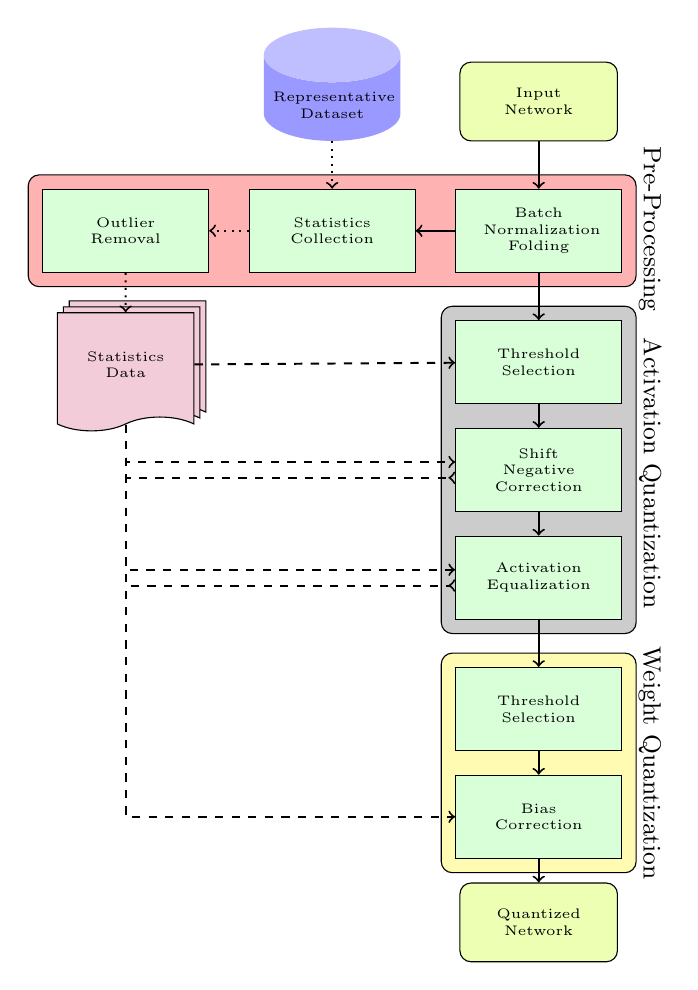
\begin{tikzpicture}[font=\small,every label/.append style={font=\small,align=center}]
\node (net) [startstop,font=\tiny,text width=1.4cm] {Input Network};
        \node[below=0.6cm of net,block,fill=green!15, text width=1.4cm,font=\tiny,align=center] (bf) {Batch\\Normalization Folding};

        \node[below=0.6cm of bf,block,fill=green!15, text width=1.4cm,font=\tiny,align=center] (at) {Threshold Selection};
       
        \node[below=0.3cm of at,block,fill=green!15, text width=1.4cm,font=\tiny,align=center] (snc) {Shift\\Negative Correction};
        \node[below=0.3cm of snc,block,fill=green!15, text width=1.4cm,font=\tiny,align=center] (ae) {Activation Equalization};
\node[left=0.5cm of bf,block,fill=green!15, text width=1.4cm,font=\tiny,align=center] (sc) {Statistics Collection};
        
         \node[left=0.5cm of sc,block,fill=green!15, text width=1.4cm,font=\tiny,align=center] (zs) {Outlier Removal};
        \node[below=0.5cm of zs,tape, draw,thin, tape bend top=none,fill=purple!20,double copy shadow,minimum height=1.5cm, text width=1.5cm,font=\tiny,align=center](sd) {Statistics Data};
        \node[above=0.6cm of sc,cylinder, cylinder uses custom fill, cylinder end fill=blue!25, cylinder body fill=blue!40,shape border rotate=90, aspect=0.4,minimum width=1cm,minimum height=1.4cm, text width=1.5cm,align=center,font=\tiny](ds) {Representative Dataset };
        
        
        \node[below=0.6cm of ae,block,fill=green!15, text width=1.4cm,font=\tiny,align=center] (wt) {Threshold Selection};
        \node[below=0.3cm of wt,block,fill=green!15, text width=1.4cm,font=\tiny,align=center] (bc) {Bias\\Correction};


        \node (qnet) [startstop,below=0.3cm of bc,font=\tiny,text width=1.4cm] {Quantized Network};
        \begin{pgfonlayer}{background}
            \node[draw,rounded corners,fit=(at) (ae) (snc),fill=black!20,inner sep=5pt,label={[label distance=-1.8cm,text depth=0.4cm,rotate=-90] right:{Activation Quantization}}](fit2){};
            \node[draw,rounded corners,fit=(wt) (bc),fill=yellow!30,inner sep=5pt,label={[label distance=-1.6cm,text depth=0.4cm,rotate=-90] right:{Weight Quantization}}](fit2){};
            \node[draw,rounded corners,fit=(bf) (zs) (sc),fill=red!30,inner sep=5pt,label={[label distance=-1.2cm,text depth=0.4cm,rotate=-90] right:{Pre-Processing}}](fit2){};
        \end{pgfonlayer}
        \node[dummy,below=0.825 of ae] (d) {};
        
\draw[->,dotted,line width=0.25mm] (zs)  -- (sd);
\draw[->,dashed,line width=0.25mm](sd) |- ([yshift=0.1cm] snc.west);
        \draw[-<,dashed,line width=0.25mm](sd) |- ([yshift=-0.1cm] snc.west);
        
        \draw[->,dashed,line width=0.25mm](sd) -- (at);
        \draw[->,dashed,line width=0.25mm](sd) |- ([yshift=0.1cm]ae.west);
        \draw[-<,dashed,line width=0.25mm](sd) |- ([yshift=-0.1cm]ae.west);
        
        \draw[->,dashed,line width=0.25mm](sd) |- (bc);


        \draw[->,line width=0.25mm] (net) -- (bf);    
\draw[->,line width=0.25mm] (bf) -- (sc);
        \draw[->,line width=0.25mm] (bf) -- (at);
        \draw[->,line width=0.25mm] (at) -- (snc);
        \draw[->,line width=0.25mm] (snc) -- (ae);
        \draw[->,line width=0.25mm] (ae) -- (wt);
        \draw[->,line width=0.25mm] (wt) -- (bc);
        \draw[->,line width=0.25mm] (bc) -- (qnet);
        
        \draw[->,dotted,line width=0.25mm] (sc) -- (zs);
        \draw[->,dotted,line width=0.25mm] (ds) -- (sc);
    \end{tikzpicture}
    \caption{The HPTQ framework. Dashed lines represent statistical information passing, which include also their updates, dotted lines represent data passing and solid lines represent an updated network. }
    \label{fig:cptq_flow}
\end{figure}
 




\subsection{Pre-Processing}
The pre-processing stage consists of folding batch normalization layers into their preceding convolution layers \cite{jacob2018quantization}, collecting activation statistics using the representative dataset and finally removing outliers from the collected statistics. 

\paragraph{Batch-Normalization Folding.} 
A common technique to reduce model size and computational complexity is batch-normalization folding \cite{jacob2018quantization} (also known as batch-normalization fusing) in which batch-normalization layers are folded into the weights of their preceding convolution layers. 

\paragraph{Statistics Collection.}
In this stage we infer all of the samples in the representative dataset  and collect activation statistics of each layer. Specifically, for each layer  denote the collection of its activations over  by .
Based on  we collect histograms for each tensor as well as the minimum, maximum and mean values per channel. In the reset of this work we assume that activation tensors   have three dimensions where ,  and  are the height, weight and number of channels, respectively.

\paragraph{Outlier Removal.}
In this step we filter out outliers in the activation histograms using the z-score approach described in \cite{aggarwal2015outlier}. 
Specifically, we remove histogram bins for which the absolute z-score value is larger than a predefined threshold. This implies that we restrict the range of each histogram bin to a predefined number of standard deviations from its activation mean value. 
See Figure \ref{fig:z_score} for an example.
Note that since this step updates the histograms, it applies only to the Threshold Selection step (see Figure \ref{fig:cptq_flow}).



\begin{figure}[H]
     \centering
     \includegraphics[scale=0.3]{images/outlier_removal.png}
     \caption{Outlier Removal. Left: an input data distribution. Middle: the respective distribution of absolute z-score values. Right: data distribution after outlier removal.}
     \label{fig:z_score}
\end{figure}
 

\subsection{Activation Quantization}
This stage consists of three steps: threshold selection, shift negative correction (SNC) and activation equalization.  
In the threshold selection step, we set power-of-two thresholds per tensor. The SNC step is a trick that improves the quantization of signed activation functions with a small negative range \cite{bhalgat2020lsq+}. 
In the activation equalization step we equalize the expected dynamic ranges of activation channels by applying a modified version of a technique that appears in \cite{nagel2019data}. 






\paragraph{Threshold Selection.}   



Given a fixed bit width , our aim is to find a power-of-two threshold  that minimizes the noise caused by the quantization of each layer  in the network. Formally, for each layer  in the network, our objective is to find a threshold  that minimizes 

where  is the size of the representative dataset,  is the collection of activation tensors in the -th layer and  is some error measurement.




In an ablation study we examine the effect of several possible quantization error measurements on the actual task accuracy, including  Norms \cite{nahshan2019loss} and Kullback–Leibler (KL) divergence \cite{szymon}.
Our results show that Mean Square Error (MSE) \cite{nahshan2019loss} achieves the best performance (see Table \ref{tab:activation_t}). 
Thus, the objective of the threshold selection is to minimize










In practice, we approximate a solution to this minimization problem by estimating the noise based on the histogram corresponding to layer  collected in the Statistics Collection step above. The restriction of the threshold to power-of-two values implies that the search space is discrete. 
Let   be the maximal absolute value of an activation in  over the representative dataset  that was collected in the Statistics Collection step above and define the no-clipping threshold:
  
Note that the clipping noise induced by the threshold  is zero and that for any power-of-two threshold larger than , the noise is increased.
Thresholds smaller than  may reduce the noise, albeit, at the cost of increasing the clipping noise. 
Therefore, we search for a threshold minimizing the quantization error starting with  and iteratively decreasing it (see. Algorithm \ref{alg:threshold_selection}).

\begin{algorithm}[H]\label{alg:threshold_selection}
 \KwData{quantization error estimator ERR ; no-clipping threshold ; bit-width ;  iterations}
 \KwResult{ threshold value }
  \;
   \;
 \For{i in 0 to n}{
   \;
   \;
  \If{}{
     \; 
    
  }
 }
 return 
 \caption{Constraint threshold selection}
\end{algorithm}












\paragraph{Shift Negative Correction (SNC).}  
Recent works have shown benefits in using signed, non-linear activation functions, such as Swish \cite{ramachandran2017searching}, PReLU and HSwish \cite{howard2019searching}. However, a signed symmetric quantization of these functions can be inefficient due to differences between their negative and positive dynamic ranges.
The main idea in SNC is to reduce the quantization noise of an unsigned activation function with a small negative range (relatively to its positive range). 
This is done by adding a positive constant to the activation values (shifting its values) and using an unsigned quantizer with the same threshold. This effectively doubles the quantization grid resolution.
Note that shifting the values can imply added clipping noise on the one hand but reduced rounding noise on the other.

This step can be viewed as an adaptation to PTQ of a technique that appears in \cite{bhalgat2020lsq+}, where activations are shifted and scaled in order to match a given dynamic range of a quantizer. Here, we do not add scaling due to its implied added complexity.
Specifically, let  be the activation function in some layer  in the network, let  be its threshold, calculated in the Threshold Selection step above and let
 
be its minimal (negative) activation value over the representative dataset , collected in the Statistics Collection step above.
If  for a hyperparameter , then we replace  with a shifted version  and replace the signed quantizer with an unsigned quantizer followed by another shift operation as follows:

where  is the signed quantizer,  is the unsigned quantizer and  is the bit-width.
In practice, the last subtraction of  is folded into the following operation in the network.




\paragraph{Activation Equalization.} 
In this step, we equalize activation ranges per channel similarly to the methods presented in \cite{nagel2019data,meller2019same}. 
Here, we set the scale-per-channel factor according to the value of the threshold that is selected per-tensor. The motivation to use this scaling factor in order to equalize the activation ranges is to use the maximum range of the quantization bins for each channel (see Figure \ref{fig:channels_corr}).



The authors in \cite{nagel2019data, meller2019same} suggest to perform channel equalization by exploiting the positive scale equivariance property of activation functions. 
It holds for any piece-wise linear activation function in its relaxed form:

where  is a piece-wise linear function,  is its modified version that fits this requirement and  is a diagonal matrix with  denoting the scale factor for channel .

The positive scaling equivariance can be applied on the following set of consecutive layers: a linear operation, a piece-wise linear function  and an additional linear operation. This is demonstrated in the following equation:

where  and  are the first layer's weights and bias,  and  are the second layer's  weights and bias. Although Eq. \ref{eq:equalization}  demonstrates the case of fully-connected layers, it can be also extended for CNNs where the scaling is performed per channel.

We present a use case of channel equalization named \textit{Max Channel Equalization} which can be applied in any quantization scheme.
We assume that  is one of the following non-linear functions: ReLU, ReLU8 or PReLU. Given the quantization threshold  of a non-linear function as well as the maximal activation value of the  channel  , where  is the activation tensor of the  layer, we set:

so that the maximal value of each channel in tensor  will be the threshold value (see Figure \ref{fig:channels_corr}).




\begin{figure}[H]
    \centering
    \includegraphics[scale=0.22]{images/act_scale_v2.png}
    \caption{
    An example of Max Channel Equalization using \mbvtwo. 
    Left: the max value  of each channel.
    Middle: the inverse scale factor  for each channel .
    Right: the max value of each channel after equalization using this scaling factor.
    }
    \label{fig:channels_corr}
\end{figure}



\subsection{Weight Quantization}
In the Weight Quantization stage we quantize the network's weights.
It was shown in \cite{krishnamoorthi2018quantizing,rastegari2016xnor} that weight quantization with scaling per channel improves accuracy.
Moreover, this work presents an efficient dot product and convolution implementation supporting per-channel quantization. 
Our Weight Quantization stage consists of per-channel threshold selection and bias correction \cite{nagel2019data}.




\paragraph{Threshold Selection.} 
As noted above, weight quantization is performed per-channel. Its thresholds are selected similarly to activation thresholds (see Algorithm \ref{alg:threshold_selection}). However, a key difference is that here the search is performed directly on the weight values, opposed to the statistical values that are used for activation.
More precisely, given the weights  of some channel in the network, the initial no-clipping threshold is 

where  are the entries of . 
Additionally, the error induced by a threshold  is
 
Note that as with activations, MSE is selected as an error measurement since it yields the best performance (see Table \ref{tab:weights_t}). 














\paragraph{Bias Correction.} Quantization of weights induce bias shifts to activation means that may lead to detrimental behaviour in the following layers \cite{nagel2019data,finkelstein2019fighting}.  
Explicitly, let  be the floating point output of a fully connected layer where  are the floating-point input activation, weight and bias, respectively. 
Denote the quantized weights of the layer by 
and the corresponding output by
.
The induced bias shift  can be expressed as follows:

Several works propose approaches to correct the quantization induced bias. 
These include using batch-normalization statistics \cite{nagel2019data}, micro training  \cite{finkelstein2019fighting} and applying scale and shift per channel \cite{NEURIPS2019_c0a62e13}.

We adopt the solution in \cite{nagel2019data}, in which the bias shift is fixed by modifying the layer's bias vector

where  is the per channel empirical mean obtain in the Statistic Collection stage above. 
Note that although the above is written for a fully connected layer, it applies to convolutional layers as well, as shown in \cite{nagel2019data}.


 \section{Experimental Results}\label{sec:experimental}
In this section we evaluate the performance of HPTQ with 8-bit quantization over different tasks and a variety of network architectures. 
The experiments are divided into two parts. The first part presents an overall performance comparison to the floating point baseline as well as to state-of-the-art quantization approaches. The second part presents an ablation study that analyzes the influence of each technique in HPTQ separately.





\subsection{Overall Performance Evaluation}
We evaluate the performance of HPTQ on four different tasks: image classification, object detection, semantic segmentation and pose estimation.
For each task, we present a comparison between the performance of models quantized by HPTQ and their floating point baselines. Furthermore, for classification and segmentation we provide a comprehensive performance comparison of HPTQ with both PTQ and QAT state-of-the art quantization methods.

We use the same set of hyper-parameters for all our experiments.
Specifically, the number of image samples in the representative dataset  is 500. 
The z-score threshold in the outlier removal step is .
The SNC threshold is . 
Last, for both activations and weights, the number of iterations performed in Algorithm \ref{alg:threshold_selection} in the threshold selection search is set to . One should note that fine-tuning the hyper-parameters per network may lead to further improvement.
In all of the tables below  is the difference between the performance of the floating point model and the quantized model, \textit{PC} indicates the use of weights per channel quantization and \textit{PoT} indicates power-of-two thresholds.





\paragraph{Classification.} 
We evaluate HPTQ on the ImageNet classification task \cite{deng2009imagenet}  using \mbvone, \mbvtwo and \res architectures\footnote{\url{https://www.tensorflow.org/api_docs/python/tf/keras/applications}}. 
Tables \ref{table:mbv1_com}, \ref{table:mbv2_com} and \ref{table:res_com} present comparisons of HPTQ with other quantization methods, both PTQ and QAT, for the three architectures. The results show that HPTQ achieves competitive performance despite the hardware friendly constraints.
In the tables below \textit{F-Acc} is the floating point accuracy and \textit{Q-Acc} is the accuracy of the quantized model.


\begin{table}[H]
\centering
\caption{ImageNet classification \cite{deng2009imagenet} with \mbvone  }
\label{table:mbv1_com}
\begin{tabular}{|c|l|c|c|l|l|l|}
\hline
\multicolumn{1}{|c|}{\textbf{Type}}                                           & \multicolumn{1}{|c|}{\textbf{Method}}          & \multicolumn{1}{|c|}{\textbf{PC}}              & \multicolumn{1}{|c|}{\textbf{PoT}}        & \multicolumn{1}{|c|}{\textbf{F-Acc}} & \multicolumn{1}{|c|}{\textbf{Q-Acc}} & \multicolumn{1}{|c|}{\textbf{}} \\ \hline
\multirow{2}{*}{\rotatebox[origin=c]{90}{QAT}} & \qt             & \xmark      & \xmark     & 70.9  & 70.0    & 0.9      \\ \cline{2-7} 
                                               & \tqt            & \xmark      & \checkmark & 71.1  & 71.1  & 0.0        \\ \hline
\multirow{5}{*}{\rotatebox[origin=c]{90}{PTQ}} & \ssbd           & \xmark      & \xmark     & 70.9  & 69.95 & 0.95     \\ \cline{2-7} 
                                               & \Krishnamoorthi & \checkmark  & \xmark     & 70.9  & 70.3  & 0.6      \\ \cline{2-7} 
                                               & \wu             & \checkmark  & \xmark     & 71.88 & 70.39 & 1.49     \\ \cline{2-7} 
                                               & \lee            & \xmark      & \xmark     & 69.5  & 68.84 & 0.66     \\ \cline{2-7} 
                                               & \textbf{\cptq}           & \checkmark  & \checkmark & \textbf{70.55} & \textbf{70.41} & \textbf{0.14}     \\ \hline
\end{tabular}
\end{table}


\begin{table}[H]
\centering
\caption{ImageNet classification \cite{deng2009imagenet} with \mbvtwo}
\label{table:mbv2_com}
\begin{tabular}{|c|l|c|c|l|l|l|}
\hline
\multicolumn{1}{|c|}{\textbf{Type}}                                           & \multicolumn{1}{|c|}{\textbf{Method}}          & \multicolumn{1}{|c|}{\textbf{PC}}              & \multicolumn{1}{|c|}{\textbf{PoT}}        & \multicolumn{1}{|c|}{\textbf{F-Acc}} & \multicolumn{1}{|c|}{\textbf{Q-Acc}} & \multicolumn{1}{|c|}{\textbf{}} \\ \hline
\multirow{3}{*}{\rotatebox[origin=c]{90}{QAT}}  & \qt                     & \xmark          & \xmark     & 71.9                   & 70.9   & 1.0        \\ \cline{2-7} 
                                                & \rvquant                & \xmark          & \xmark     & 70.10                 & 70.29 & -0.19    \\ \cline{2-7} 
                                                & \tqt                    & \xmark          & \checkmark & 71.7                   & 71.8   & -0.10     \\ \hline
\multirow{10}{*}{\rotatebox[origin=c]{90}{PTQ}} & \adaquant               & \xmark      & \xmark     & 73.03                  & 73.03  & 0.0        \\ \cline{2-7} 
                                                 & \zeroq                  & \xmark      & \xmark     & 73.03                  & 72.91  & 0.12     \\ \cline{2-7} 
                                                & \ssbd                   & \xmark        & \xmark     & 71.9                   & 71.29  & 0.61     \\ \cline{2-7} 
                                                & \wu                     & \checkmark     & \xmark     & 71.88                  & 71.14  & 0.74     \\ \cline{2-7} 
                                                & \Krishnamoorthi         & \checkmark      & \xmark     & 71.9                   & 69.7   & 2.2      \\ \cline{2-7} 
                                                & \multirow{2}{*}{\nagel} & \xmark          & \xmark     & \multirow{2}{*}{71.72} & 70.99  & 0.73     \\ \cline{3-4} \cline{6-7} 
                                                &                         & \checkmark      & \xmark     &                        & 71.16  & 0.56     \\ \cline{2-7} 
                                                & \dfq                    & \xmark          & \xmark     & 71.72                  & 70.92  & 0.8      \\ \cline{2-7} 
                                                & \lee                    & \xmark          & \xmark     & 71.23                  & 69.5   & 1.73     \\ \cline{2-7} 
                                                & \textbf{\cptq}                   & \checkmark      & \checkmark & \textbf{71.812}                 & \textbf{71.46}  & \textbf{0.352}    \\ \hline
\end{tabular}
\end{table}


\begin{table}[H]
\centering
\caption{ImageNet classification \cite{deng2009imagenet} with \res}
\label{table:res_com}
\begin{tabular}{|c|l|c|c|l|l|l|}
\hline
\multicolumn{1}{|c|}{\textbf{Type}}                                           & \multicolumn{1}{|c|}{\textbf{Method}}          & \multicolumn{1}{|c|}{\textbf{PC}}              & \multicolumn{1}{|c|}{\textbf{PoT}}        & \multicolumn{1}{|c|}{\textbf{F-Acc}} & \multicolumn{1}{|c|}{\textbf{Q-Acc}} & \multicolumn{1}{|c|}{\textbf{}} \\ \hline
\multirow{6}{*}{\rotatebox[origin=c]{90}{QAT}}  & \qt                              & \xmark         & \xmark     & 76.4                   & 74.9   & 1.5      \\ \cline{2-7} 
                                                & \rvquant                         & \xmark         & \xmark     & 75.92                  & 75.67  & 0.25     \\ \cline{2-7} 
                                                & \hawq                            & \checkmark    & \xmark     & 77.72                  & 77.58  & 0.14     \\ \cline{2-7} 
                                                & \lsq                             & \xmark          & \xmark     & 76.9                   & 76.8   & 0.1      \\ \cline{2-7} 
                                                & \tqt                             & \xmark          & \checkmark & 76.9                   & 76.5   & 0.4      \\ \cline{2-7} 
                                                & \faq                             & \xmark          & \xmark     & 75.4                   & 75.4   & 0.0        \\ \hline
 \multirow{10}{*}{\rotatebox[origin=c]{90}{PTQ}} & \zeroq                           & \xmark      & \xmark     & 77.72                  & 77.67  & 0.05     \\ \cline{2-7} 
                                                & \ocs                             & \xmark         & \xmark     & 76.1                   & 75.9   & 0.2      \\ \cline{2-7} 
                                                & \ssbd                            & \xmark          & \xmark     & 75.2                   & 74.95  & 0.25     \\ \cline{2-7} 
                                                & \he                              & \xmark          & \xmark     & 75.3                   & 75.03  & 0.27     \\ \cline{2-7} 
                                                & \wu                              & \checkmark     & \xmark     & 76.16                  & 76.05  & 0.11     \\ \cline{2-7} 
                                                & \multirow{2}{*}{\nagel}          & \xmark         & \xmark     & \multirow{2}{*}{76.07} & 75.87  & 0.2      \\ \cline{3-4} \cline{6-7} 
                                                &                                  & \checkmark      & \xmark     &                        & 75.88  & 0.19     \\ \cline{2-7} 
                                                & \multirow{2}{*}{\Krishnamoorthi} & \xmark         & \xmark     & \multirow{2}{*}{75.2}  & 75.00     & 0.20      \\ \cline{3-4} \cline{6-7} 
                                                &                                  & \checkmark     & \xmark     &                        & 75.1   & 0.1      \\ \cline{2-7} 
                                                & \textbf{\cptq}                            & \checkmark      & \checkmark & \textbf{75.106}                 & \textbf{75.018} & \textbf{0.088}    \\ \hline
\end{tabular}
\end{table}

\paragraph{Semantic Segmentation.}
We evaluate HPTQ on Pascal VOC \cite{everingham2010pascal} using DeepLab V3\footnote{\url{https://github.com/tensorflow/models/blob/master/research/deeplab/g3doc/model_zoo.md}} \cite{chen2017rethinking} with \mbvtwo as a backbone. Table \ref{tab:deeplab} shows that HPTQ achieves competitive results compared to other PTQ methods.

\begin{table}[H]
\caption{Semantic segmentation on Pascal VOC \cite{everingham2010pascal} using DeepLab V3 with \mbvtwo as a backbone. \textit{F-mIoU} is the floating point  mean Intersection-over-Union (mIoU) and \textit{Q-mIoU} is the mIoU of the quantized model.}
\label{tab:deeplab}
\centering
\begin{tabular}{|c|l|c|c|l|l|l|}
\hline
\multicolumn{1}{|c|}{\textbf{Type}}                                           &  \multicolumn{1}{|c|}{\textbf{Method}}                  &  \multicolumn{1}{|c|}{\textbf{PC}}             &  \multicolumn{1}{|c|}{\textbf{PoT}}        &  \multicolumn{1}{|c|}{\textbf{F-mIoU}}                  & \multicolumn{1}{|c|}{\textbf{Q-mIoU}} & \multicolumn{1}{|c|}{\textbf{}} \\ \hline
\multirow{4}{*}{\rotatebox[origin=c]{90}{PTQ}} & \dfq                    & \xmark      & \xmark     & 72.45                  & 72.33 & 0.12     \\ \cline{2-7} 
                                               & \multirow{2}{*}{\nagel} & \xmark     & \xmark     & \multirow{2}{*}{72.94} & 72.44 & 0.50      \\ \cline{3-4} \cline{6-7} 
                                               &                         & \checkmark  & \xmark     &                        & 72.27 & 0.67     \\ \cline{2-7} 
                                               & \textbf{\cptq}                   & \checkmark  & \checkmark & \textbf{75.57}                  & \textbf{75.38} & \textbf{0.19}     \\ \hline
\end{tabular}
\end{table}












\paragraph{Object Detection.} 
We evaluate HPTQ on COCO  \cite{lin2014microsoft} using the SSD detector \cite{liu2016ssd} with several backbones\footnote{\url{https://github.com/tensorflow/models/blob/master/research/object_detection/g3doc/tf2_detection_zoo.md}}. 
HPTQ achieves similar Mean Average Precision (mAP) to the floating point baseline as demonstrated in Table  \ref{table:det}.


\begin{table}[H]
\centering
\caption{Object detection results with HPTQ on COCO  \cite{lin2014microsoft} using \mbvtwo and \res as backbones. \textit{F-mAP} is the floating point mAP  and \textit{Q-mAP} is the mAP of the quantized model.}
\label{table:det}
\begin{tabular}{|l|l|l|}
\hline
\multicolumn{1}{|c|}{\textbf{Model}}                           & \multicolumn{1}{|c|}{\textbf{F-mAP}} & \multicolumn{1}{|c|}{\textbf{Q-mAP}} \\ \hline
SSD \mbvtwo 320x320  & 20.2  & 20.21     \\ \hline
SSD  \mbvtwo FPN Lite 320x320        & 22.2  & 21.93     \\ \hline
SSD \res V1 FPN 640x640     & 34.3  & 34.3      \\ \hline
\end{tabular}
\end{table}





\paragraph{Pose-Estimation.} 
We evaluate HPTQ on the single-person pose estimation task using LPN network \cite{zhang2019simple} on the LIP (Look into Person) dataset \cite{liang2018look}. 
We use the PCKh metric \cite{liang2018look} for evaluation, which is the head-normalized probability of correct keypoints. 
HPTQ achieves similar performance to the floating point baseline with only a slight degradation from 81.65 to 81.53 PCKh.




\subsection{Ablation Study}\label{sec:ablation}

We provide an ablation study of HPTQ's performance on the ImageNet classification task \cite{deng2009imagenet} using eleven networks\footnote{\url{https://www.tensorflow.org/api_docs/python/tf/keras/applications}}. 
The study is divided into two parts analyzing activation quantization and weight quantization. 

Table \ref{table:atype_effect} compares the performance of HPTQ between four cases: full floating-point, activation quantization, weight quantization and joint quantization of both. 
The comparison shows that activation quantization causes a larger degradation in performance compared to weight quantization, especially for EfficientNet with Swish activations functions. 
This might be due to the fact that activation equalization is not applied for these activations.



\begin{table}[H]
\centering
\caption{ImageNet classification \cite{deng2009imagenet} accuracy with HPTQ in four cases: full floating-point, activation quantization, weight quantization and both activation and weight quantization.}
\label{table:atype_effect}
\begin{tabular}{|l|l|l|l|l|}
\hline
\multicolumn{1}{|c|}{\textbf{Network}} & \multicolumn{1}{c|}{\textbf{F-Acc}} & \multicolumn{1}{c|}{\textbf{\begin{tabular}[c]{@{}c@{}}Q-Acc \\ (Activation)\end{tabular}}} & \multicolumn{1}{c|}{\textbf{\begin{tabular}[c]{@{}c@{}}Q-Acc \\ (Weights)\end{tabular}}} & \multicolumn{1}{c|}{\textbf{\begin{tabular}[c]{@{}c@{}}Q-Acc\\  (Both)\end{tabular}}} \\ \hline
\mbvone        & 70.558 & 70.48 & 70.394 & 70.418          \\ \hline
\mbvtwo        & 71.812 & 71.616 & 71.668       & 71.46           \\ \hline
\nasnet        & 74.376 & 74.068 & 74.352       & 73.888          \\ \hline
\vgg           & 70.956 & 70.834 & 70.946       & 70.81           \\ \hline
\inc           & 77.908 & 77.872 & 77.844       & 77.85           \\ \hline
\incres        & 80.284 & 80.154 & 80.32       & 80.14           \\ \hline
\res           & 75.106 & 75.072 & 75.06       & 75.018          \\ \hline
\eff           & 77.2   & 74.3 & 77.012       & 74.216          \\ \hline
\effrelu       & 77.65  & 77.1 & 77.568       & 77.092         \\ \hline
\dense         & 74.848 & 73.252 & 74.784       & 73.356          \\ \hline
\xecption      & 79.05  & 79.048 & 79.062       & 78.972          \\ \hline
\end{tabular}
\end{table}


\paragraph{Activation Quantization Analysis.}
In this analysis we evaluate the influence of the different methods used for quantizing the activations (without quantizing the weights). 
The analysis is performed with eleven different network architectures\footnote{\label{foot:eff}EfficientNet-B0 ReLU is a trained version of EfficientNet-B0 with ReLU activation function instead of swish}\footnote{ \url{https://keras.io/api/applications/}} on the ImageNet classification \cite{deng2009imagenet} task.
Table \ref{tab:activation_t} shows an accuracy comparison using four different threshold selection methods without applying any other of the activation quantization steps. 
NC indicates using the no-clipping threshold. Mean Square Error (MSE), Mean Average Error (MAE) and Kullback–Leibler (KL) are three different error measurements  in Equation \ref{equ:err}.

\begin{table}[H]
\caption{ImageNet classification \cite{deng2009imagenet} accuracy with activations quantized using different threshold selection methods (weights are in floating point).
}
\label{tab:activation_t}
\begin{tabular}{|l|l|l|l|l|}
\hline
\multicolumn{1}{|c|}{\textbf{Network}}           &  \multicolumn{1}{|c|}{\textbf{NC}}       & \multicolumn{1}{|c|}{\textbf{MSE}}    & \multicolumn{1}{|c|}{\textbf{MAE}}    & \multicolumn{1}{|c|}{\textbf{KL}}   \\ \hline
\mbvone           & 70.406  & 70.434 & 60.218 & 70.418   \\ \hline
\mbvtwo           & 71.25 & 71.458 & 65.918  & 71.482   \\ \hline
\vgg              & 70.8 & 70.764 & 58.37 & 65.096   \\ \hline
\res              & 74.612 & 74.996 & 67.896 & 59.556  \\ \hline
\end{tabular}
\centering
\end{table}

Table \ref{table:activation_ablation} shows the incremental accuracy influence on ImageNet classification \cite{deng2009imagenet} of the methods used by HPTQ for activation quantization (without quantizing weights).
Note that SNC is applied in all of the experiments in the table and its influence is studied separately below.
The table shows that all of the methods result in an improvement. Note that fine-tuning the z-score threshold  per network may lead to further improvement.


\begin{table}[H]
\caption{
The accuracy influence of the different activation quantization methods used by HPTQ for ImageNet classification \cite{deng2009imagenet} when keeping all weights in floating point.
Baseline is quantization with no-clipping thresholds, \textit{+Eq.} means adding max channel equalization,
\textit{+MSE Th.} means replacing the no-clipping thresholds with MSE
and \textit{+z-score} means applying z-score outlier removal.
}
\label{table:activation_ablation}
\centering
\begin{tabular}{|l|l|l|l|l|l|}
\hline
\multicolumn{1}{|c|}{\textbf{Network Name}}            & \multicolumn{1}{|c|}{\textbf{Baseline}} & \multicolumn{1}{|c|}{\textbf{+Eq.}} & \multicolumn{1}{|c|}{\textbf{+MSE Th.}} & \multicolumn{1}{|c|}{\textbf{+z-score}} \\ \hline
\mbvone                 & 70.406          & 70.418                 &70.48                &    70.48            \\ \hline
\mbvtwo                 & 71.25         &   71.34               &      71.528            &      71.616           \\ \hline
\nasnet                 &   18.572       &     18.484             &  73.486              &   74.068              \\ \hline
\vgg                    &   70.8       &     70.696            &  70.888              &   70.834              \\ \hline
\inc                    &  77.658       &     77.646            &  77.832              &   77.872             \\ \hline
\incres                 & 49.132        & 49.238                &   80.014              &        80.154         \\ \hline
\res                    & 74.612         & 74.654                &   75.086              &        75.072         \\ \hline
\eff                   &   13.562        &     13.736            &  74.096               &   74.3               \\ \hline
\effrelu                &   74.298        &     76.298             &  76.956               &   77.1               \\ \hline
\dense                  &  56.08       &     55.916            &  73.28              &   73.252           \\ \hline
\xecption               &   48.718       &     48.784             &  78.87               &   79.048               \\ \hline
\end{tabular}
\end{table}

Table \ref{table:snc} shows the accuracy improvement achieved by applying Shift Negative Correction (SNC). Specifically, the table compares the performance of several versions of MobileNetV1, each with different non-linear functions, with a full flow of activation quantization.

\begin{table}[H]
\centering
\caption{ImageNet classification accuracy \cite{deng2009imagenet} using HPTQ with and without SNC of \mbvone trained with different non-linear functions.}
\label{table:snc}
\begin{tabular}{|l|l|l|l|l|l|l|}
\hline
            & \multicolumn{1}{|c|}{\textbf{Swish}}              & \multicolumn{1}{|c|}{\textbf{\begin{tabular}[c]{@{}c@{}}Leaky ReLU\\ ()\end{tabular}}}  & \multicolumn{1}{|c|}{\textbf{PReLU}}  & \multicolumn{1}{|c|}{\textbf{SELU}}   \\ \hline
Float     & 73.522                & 72.866                                 & 73.114 & 72.032 \\ \hline
Without SNC & 60.98 &71.966       & 72.548 & 69.726 \\  \hline
With SNC  & 71.146           & 72.588                                                               & 72.548 & 70.902 \\ \hline
\end{tabular}
\end{table}




\paragraph{Weight Quantization Analysis.} 
In this analysis we evaluate the influence of the different methods used for quantizing weights (without quantizing activations). 
The analysis is performed with eleven different network architectures\footnote{\ref{foot:eff}EfficientNet-B0 ReLU is a trained version of EfficientNet-B0 with ReLU activation function instead of swish}\footnote{ \url{https://keras.io/api/applications/}} on the ImageNet classification \cite{deng2009imagenet} task.

Table \ref{tab:weights_t} shows an accuracy comparison of each quantized network using four different threshold selection methods (without applying bias correction).
NC indicates using the no-clipping threshold. Mean Square Error (MSE), Mean Average Error (MAE) and Kullback–Leibler (KL) are three different error measurements  in Equation \ref{equ:err}.
Similarly to the results for activation quantization in Table \ref{tab:activation_t}, the MSE error measurement achieves the best results.



\begin{table}[H]
\caption{ImageNet classification \cite{deng2009imagenet} accuracy with weights quantized using different threshold selection methods (activations are in floating point).}
\label{tab:weights_t}
\begin{tabular}{|l|l|l|l|l|}
\hline
\multicolumn{1}{|c|}{\textbf{Network}}           &  \multicolumn{1}{|c|}{\textbf{NC}}       & \multicolumn{1}{|c|}{\textbf{MSE}}    & \multicolumn{1}{|c|}{\textbf{MAE}}    & \multicolumn{1}{|c|}{\textbf{KL}}   \\ \hline
\mbvone           & 68.75  & 68.756 & 64.242 & 64.968   \\ \hline
\mbvtwo           & 69.562 & 69.758 & 67.57  & 62.394   \\ \hline
\nasnet           & 74.188 & 74.232    & 72.79  & 73.358   \\ \hline
\vgg              & 70.944 & 70.94  & 67.486 & 70.472   \\ \hline
\inc              & 77.768 & 77.82& 70.91  & 74.28   \\ \hline
\incres           & 80.244 & 80.276  & 78.676 & 77.112   \\ \hline
\res              & 75.068 & 75.11 & 72.352 & 73.418   \\ \hline
\eff              & 76.822 & 76.822 & 75.86  & 75.554   \\ \hline
\effrelu          & 77.078 & 77.218  & 76.916 & 76.674   \\ \hline
\dense            & 74.734 & 74.736  & 72.102 & 60.17   \\ \hline
\xecption         & 79.006 & 79.006  & 77.47  & 75.374   \\ \hline
\end{tabular}
\centering
\end{table}

Table \ref{table:weights_ablation} shows the incremental accuracy influence of the two methods (per channel quantization and bias correction) used in HPTQ for weight quantization (without quantizing activations) on the ImageNet classification task \cite{deng2009imagenet}.
This table shows that both of our methods result in improvement.


\begin{table}[H]
\caption{
The incremental influence of applying per-channel threshold selection (\textit{Per ch.}) and bias correction (\textit{Bias corr.}) on ImageNet \cite{deng2009imagenet} classification accuracy.
Baseline means quantization with MSE threshold applied per tensor.
}
\label{table:weights_ablation}
\centering
\begin{tabular}{|l|l|l|l|l|l|}
\hline
\multicolumn{1}{|c|}{\textbf{Network}}             & \multicolumn{1}{|c|}{\textbf{Baseline}} & \multicolumn{1}{|c|}{\textbf{Per ch.}} & \multicolumn{1}{|c|}{\textbf{+Bias corr.}} \\ \hline
\mbvone                    & 0.966                &  68.756                 &    70.394             \\ \hline
\mbvtwo                    &   0.398              &  69.758            &      71.668           \\ \hline
\nasnet                     &     73.494          &  74.232               &  74.352               \\ \hline
\vgg                      &     70.814            &  70.94               &  70.946                \\ \hline
\inc                      &     76.42             &  77.82               &  77.844               \\ \hline
\incres                  &     80.066             &  80.276               &  80.32               \\ \hline
\res                      & 74.718                &  75.11              &        75.06          \\ \hline
\eff                       &     2.524            &  76.822             &  77.012            \\ \hline
\effrelu                   &     0.682            &  77.218             &  77.568            \\ \hline
\dense                  &     72.986              &  74.736               &  74.784             \\ \hline
\xecption                &     78.786             &  79.006               &  79.062               \\ \hline
\end{tabular}
\end{table}
 \section{Conclusions}\label{sec:conculsions}
In this work we propose HPTQ, a method for hardware-friendly post-training quantization. 
HPTQ offers a flow that adapts and synergistically combines several known quantization techniques both for weights and activations.
We extensively evaluated the performance of HPTQ on four tasks: classification, object detection, semantic segmentation and pose estimation. 
Notably, for all of the tasks we demonstrated that competitive results can be obtained under our hardware-friendly constraints of uniform and symmetric quantization with power-of-two thresholds.
In addition, we performed an ablation study in which we presented the contributions of each of the methods used by HPTQ. 


\bibliographystyle{unsrt}
\bibliography{ref}



\end{document}
